\documentclass[aspectratio=169]{beamer}
\PassOptionsToPackage{english}{babel}
\usepackage{standardslides}

\title{Restricted Boltzmann Machines}
\author{Markus Pawellek}

\begin{document}
  \selectlanguage{english}

  \begin{frame}
    \vfill
    
\includegraphics[width=\textwidth]{images/netflix-logo.jpg}
    \vfill
  \end{frame}

  \frame{\titlepage}
  \begin{frame}{Outline}
    \footnotesize
    \hfill\parbox[t][7cm][l]{0.9\textwidth}{\tableofcontents}
  \end{frame}

  \section{Introduction} % (fold)
  \label{sec:introduction}
    \begin{frame}{Introduction}
      \begin{center}
        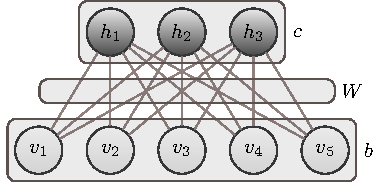
\includegraphics[height=0.35\textheight]{figures/rbm-scheme.pdf}
      \end{center}

      Why should we talk about Restricted Boltzmann Machines?
      \begin{itemize}
        \pause
        \item multiple applications in machine learning
        \pause
        \item supervised and unsupervised learning
        \pause
        \item simple and fast basic building blocks in deep learning
      \end{itemize}
    \end{frame}
  % section introduction (end)

  \section{Background} % (fold)
  \label{sec:background}
    \begin{frame}{Background}
      \begin{itemize}
        \item generative stochastic neural network that learns probability distribution
      \end{itemize}
    \end{frame}
  % section background (end)

  \section{Methodology} % (fold)
  \label{sec:methodology}
    \begin{frame}{Methodology}

    \end{frame}
  % section methodology (end)

  \section{Implementation} % (fold)
  \label{sec:implementation}
    \begin{frame}{Implementation}

    \end{frame}
  % section implementation (end)

  \section{Results} % (fold)
  \label{sec:results}
    \begin{frame}{Results}

    \end{frame}
  % section results (end)

  \section{Conclusion} % (fold)
  \label{sec:conclusion}
    \begin{frame}{Conclusion}

    \end{frame}
  % section conclusion (end)

  \begin{frame}
    \frametitle{References}
    \tiny
    \begin{multicols}{2}
      \nocite{*}
      \bibliography{references}
    \end{multicols}
  \end{frame}
\end{document}